\documentclass[a4paper,12pt]{article}
\usepackage[utf8]{inputenc}
\usepackage[spanish]{babel}
\usepackage{color}
\usepackage{parskip}
\usepackage{graphicx}
\usepackage{multirow}
\usepackage{listings}
\usepackage{vmargin}
\graphicspath{ {imagenes/} }
\definecolor{mygreen}{rgb}{0,0.6,0}
\definecolor{lbcolor}{rgb}{0.9,0.9,0.9} 
\usepackage{epstopdf}


\setpapersize{A4}
\setmargins{2.5cm}       % margen izquierdo
{1.5cm}                        % margen superior
{16.5cm}                      % anchura del texto
{23.42cm}                    % altura del texto
{10pt}                           % altura de los encabezados
{1cm}                           % espacio entre el texto y los encabezados
{0pt}                             % altura del pie de página
{2cm}     

\lstset{
backgroundcolor=\color{lbcolor},
    tabsize=4,    
%   rulecolor=,
    language=[GNU]C++,
        basicstyle=\tiny,
        aboveskip={1.5\baselineskip},
        columns=fixed,
        showstringspaces=false,
        extendedchars=false,
        breaklines=true,
        prebreak = \raisebox{0ex}[0ex][0ex]{\ensuremath{\hookleftarrow}},
        frame=single,
        showtabs=false,
        showspaces=false,
        showstringspaces=false,
        identifierstyle=\ttfamily,
        keywordstyle=\color[rgb]{0,0,1},
        commentstyle=\color[rgb]{0.026,0.112,0.095},
        stringstyle=\color{red},
        numberstyle=\color[rgb]{0.205, 0.142, 0.73},
%        \lstdefinestyle{C++}{language=C++,style=numbers}’.
}

\begin{document}
\begin{Large}
 NOMBRE:CHRISTOFER FABIÁN CHÁVEZ CARAZAS
\end{Large}


\begin{itemize}
  
 \item Escriba un programa en el cual se generen procesos y uno de ellos quede huérfano. Muestre y explique la evidencia que demuestre la existencia del proceso huerfano.


\begin{lstlisting}
int main(int argc, char *argv[]){
	pid_t pid;
	if ((pid=fork()) == 0 ){ 
		printf("1->Soy el hijo (%d, hijo de %d)\n", getpid(), getppid());
		sleep(30);
		printf("2->Soy el hijo (%d, hijo de %d)\n", getpid(), getppid());
	}
	else{ 
		printf("1->Soy el padre (%d, mi hijo es %d)\n", getpid(), pid);
		sleep(10);
		printf("2->Soy el padre (%d, mi hijo es %d)\n", getpid(), pid);
	}
	return 0;
}
\end{lstlisting}

\begin{center}
 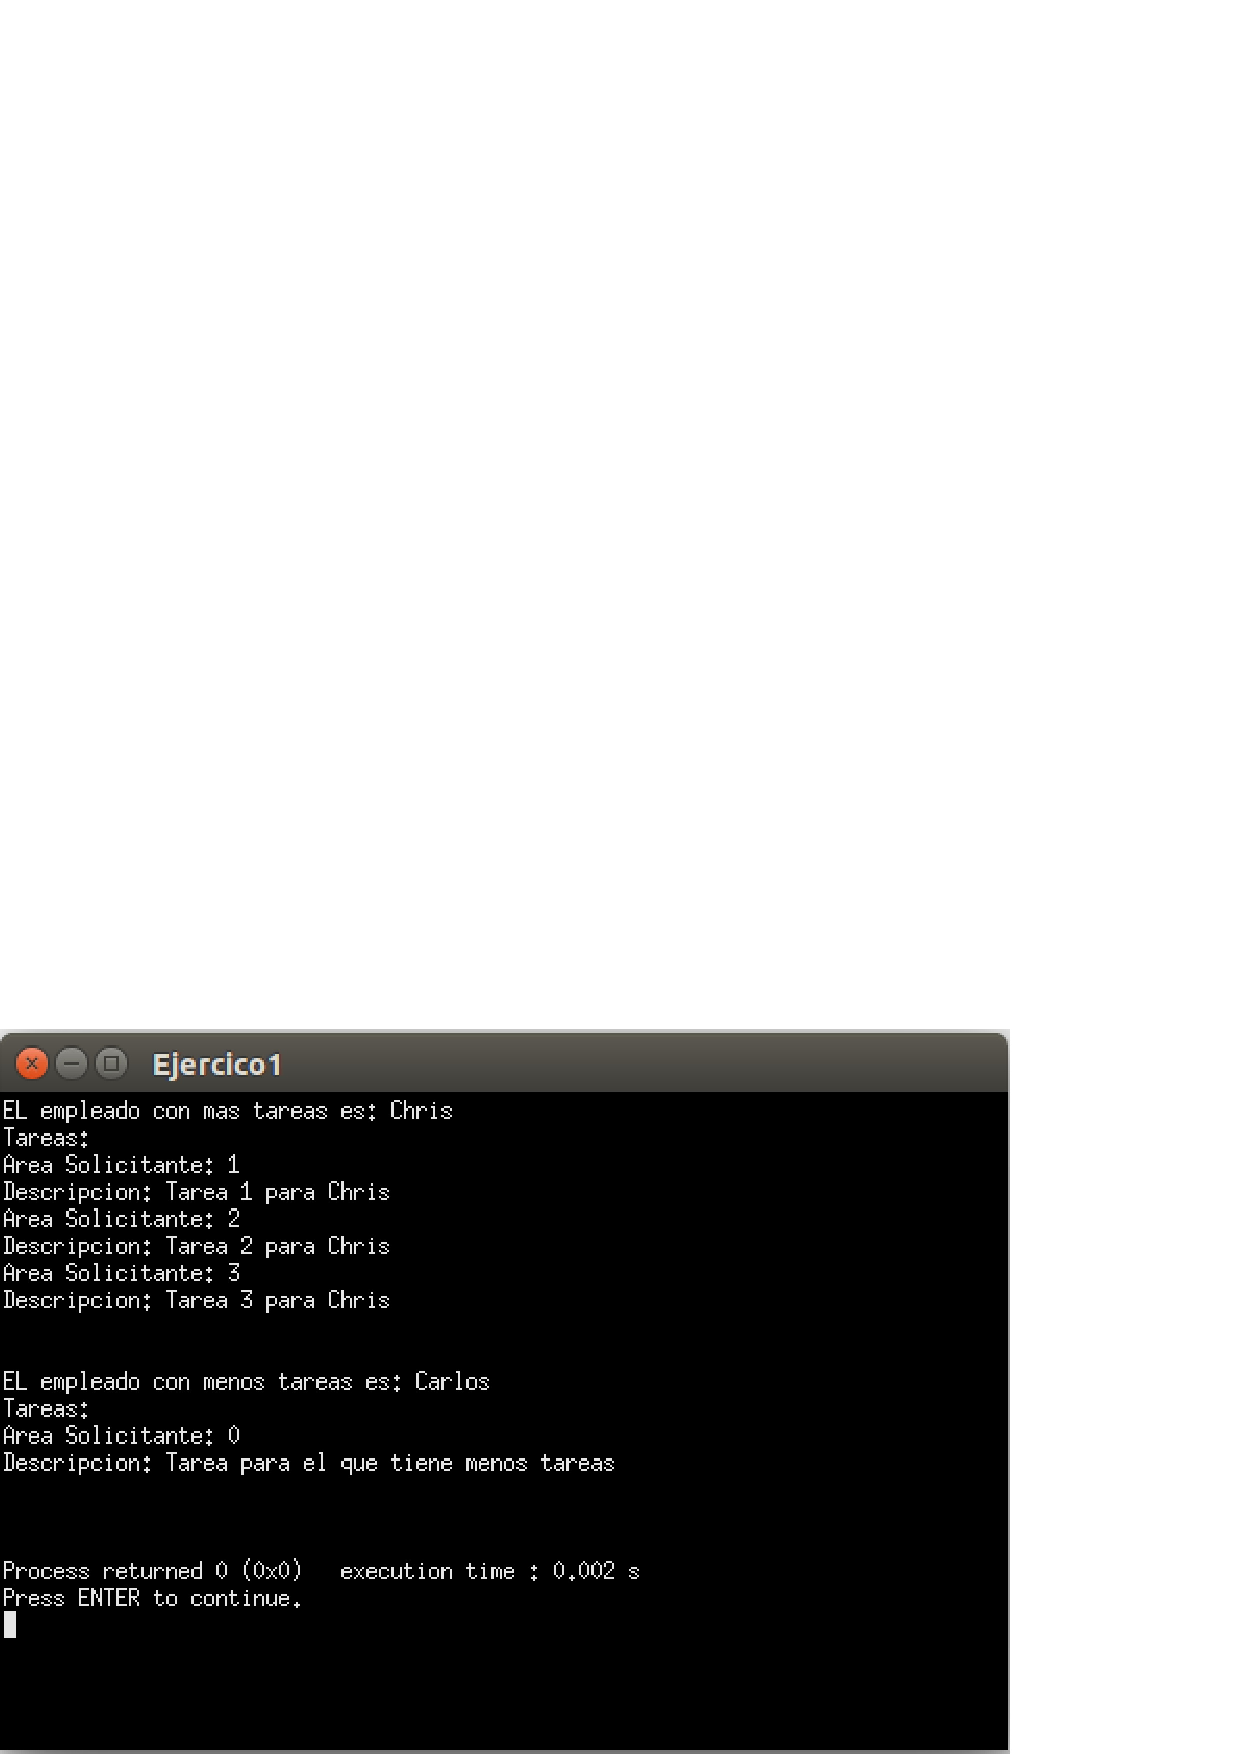
\includegraphics[scale=0.5]{1.png}
\end{center}
 

\item Escriba un programa en el cual se creen procesos y uno de ellos se encuentre en estado zombie. Muestre y explique la evidencia que demuestre la existencia del proceso zombie.

\begin{lstlisting}
int main(int argc, char *argv[]){
	pid_t pid;
	if ((pid=fork()) == 0 ){ 
		printf("1->Soy el hijo (%d, hijo de %d)\n", getpid(), getppid());
		sleep(10);
		printf("2->Soy el hijo (%d, hijo de %d)\n", getpid(), getppid());
	}
	else{ 
		printf("1->Soy el padre (%d, mi hijo es %d)\n", getpid(), pid);
		sleep(30);
		printf("2->Soy el padre (%d, mi hijo es %d)\n", getpid(), pid);
	}
	return 0;
}
\end{lstlisting}

\begin{center} 
  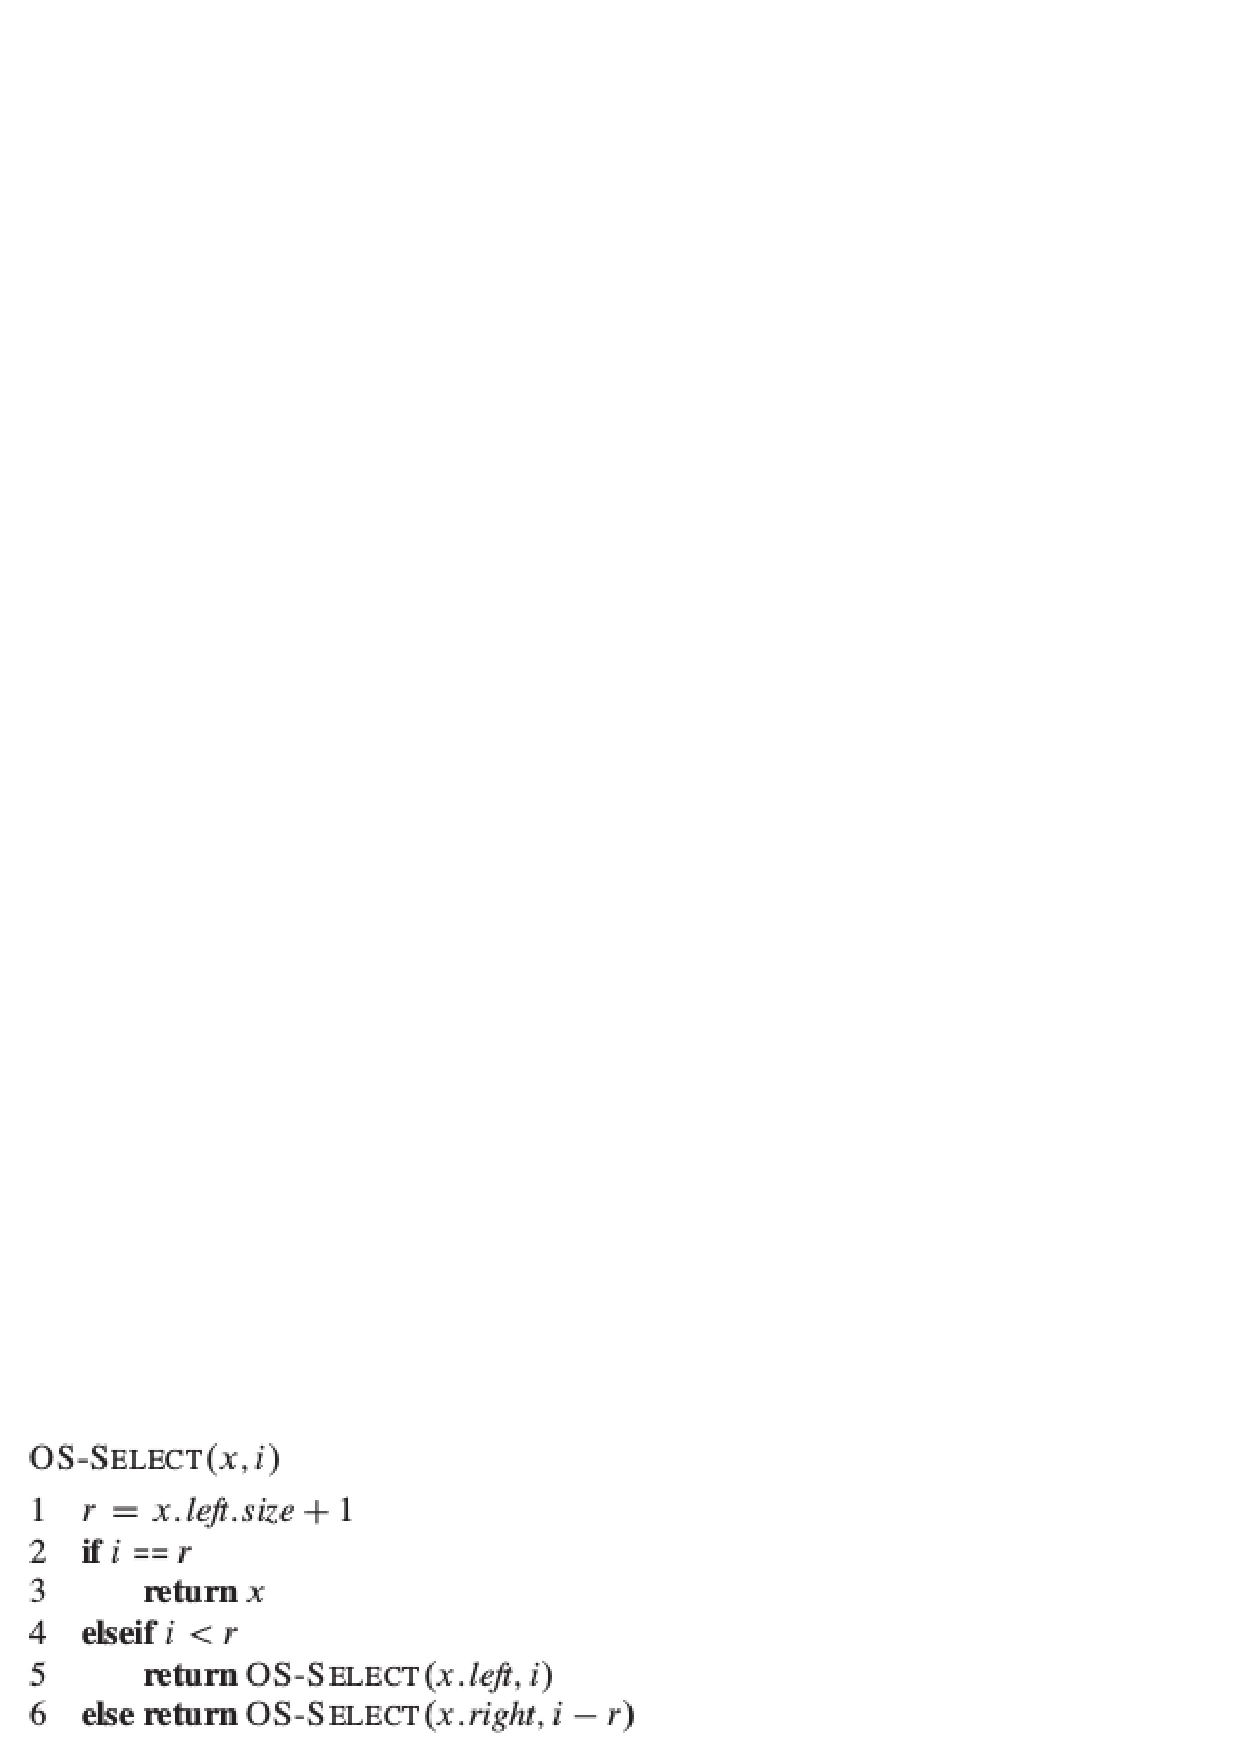
\includegraphics[scale=0.5]{2.png} 
\end{center}

\newpage

\item Escriba un programa que cree la sgte jerarquía de procesos:

\textbf{P} : el proceso padre debe de esperar a que sus hijos terminen para terminarse.

\textbf{H1} : el hijo 1, debe de mostrar su PID y el de su padre, además de enviarle cada 20 segundos una señal SIGUSR1 a H2.

\textbf{H2} : el hijo 2 se activa cuando recibe la señal de H1, y debe de mostrar su PID como respuesta a la señal SIGUSR1 que recibe, para luego volverse a suspender.

\textbf{H3} : el hijo 3 ejecuta un script que le de la bienevenida al usuario activo, considerando el horario correspondiente.

\begin{lstlisting}
#include <sys/types.h>
#include <signal.h>
#include <stdlib.h>
#include <unistd.h>
#include <stdio.h>

void alarma();
void despertar();

pid_t pidH1, pidH2 , pidH3;

int main(int argc, char *argv[]){
	int status1, status2;
	if((pidH2 = fork()) ==  0){
		while(1){
			signal(SIGUSR1,despertar);
			pause();	
		}		
	}
	else{
		if((pidH1 = fork()) == 0){
			if((pidH3 = fork()) == 0){
				system("sh script.sh");
			}
			else{
				printf("Soy el hijo1 -> %d y mi padre es %d\n",getpid(),getppid());
				signal(SIGALRM,alarma);
				alarm(20);
				while(1);
			}	
			
		}
		else{
			waitpid(pidH1,&status1,0);
			waitpid(pidH2,&status2,0);
		}
	}
}

void alarma(){
	signal(SIGALRM,SIG_IGN);
	kill(pidH2,SIGUSR1);
	signal(SIGALRM,alarma);
	alarm(20);
}

void despertar(){
	printf("Soy el hijo2 -> %d\n",getpid());
}

\end{lstlisting}

\begin{center}
 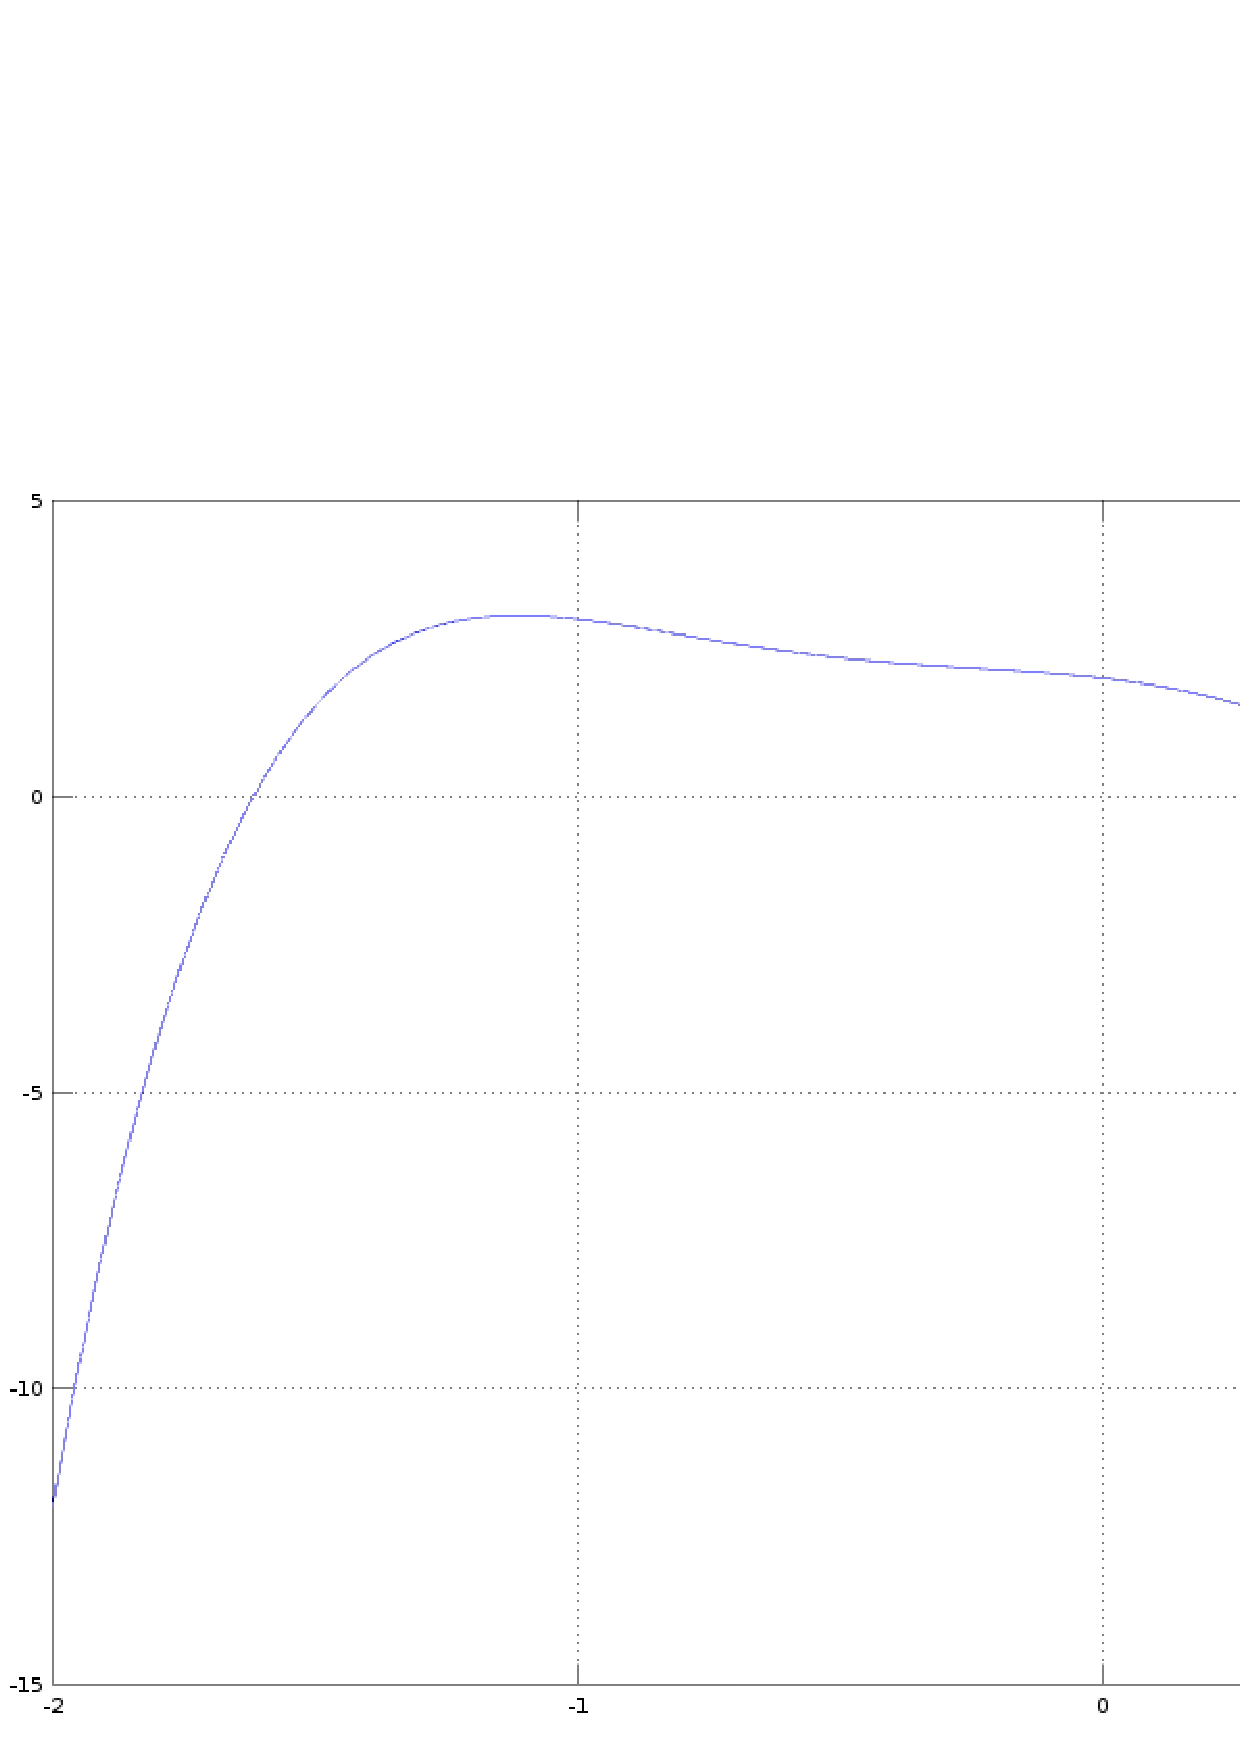
\includegraphics[scale=0.5]{3.png}
\end{center}


\end{itemize}
\end{document}
